\documentclass[11pt]{article}

\input strowpreprint

\newcommand{\kc}{\textsf{kCARTA}\xspace}

\lhead{\textsf{\textbf{DRAFT}}}

\title{kCARTA : Comparing DISORT, RTSPEC and kTWOSTREAM}

\author{Sergio De Souza-Machado, L. Larrabee Strow,\\
       Howard E. Motteler, Scott E. Hannon and Ji Gou\\
       University of Maryland Baltimore County, Baltimore, MD 21250 USA}

\begin{document}

\maketitle

\begin{abstract}
  
  Using a custom line-by-line spectroscopic code, a radiative transfer package
  using a monochromatic \textsf{SVD} compressed database has been developed. 
  Scattering computations for both downlook and
  uplook instruments can be performed using our own \textsf{kTWOSTREAM} 
  scattering code, or either of \textsf{DISORT} or \textsf{RTSPEC}.
  Here we compare the three scattering codes to each other and to actual 
  data, concentrating on the infrared window regions.

\end{abstract}

\section{Introduction}

\subsection{Spectroscopic line-by-line codes}

When using the spectra produced by spectroscopy codes in radiative transfer
algorithms, the accuracy of these codes is especially important.
For example, line mixing and far-wing effects have to be correctly and
accurately incorporated into lineshapes, as atmospheric parameters 
such as temperature and humidity as a function of atmospheric height can be
retrieved using information in spectral regions dominated by these effects. 
While these codes can be very accurate, when compared to experimentally 
obtained laboratory spectra, they are usually too slow for practical 
``on-the-fly'' applications.

One approach to implement line mixing or far wing effects is to add on a 
continuum, or to use a chi function to  multiply a Voigt or Lorentz 
lineshape. While an empirical continuum is easy to implement in a 
line-by-line code, our recent
work has shown that for water, non-Lorentz line shapes must be used
close to the line centers, a complicating factor in traditional
implementations of line-by-line codes. Similarly, line mixing effects
in between \cd lines in the 4.3 and 15 $\mu$m regions are also complicated.
These problems are not impossible to deal with, but they significantly 
complicate codes that are already difficult to develop and maintain.

The upcoming generation of nadir viewing satellite instruments for
remote sensing of atmospheric temperature and humidity profiles will
require accurate forward models for radiative transfer.  This is a
rather demanding task since these new instruments, such as the
Atmospheric InfraRed Sounder (AIRS)\cite{air:91}, have thousands of
low-noise spectral channels throughout the infrared.  Physical
retrieval algorithms using these high-resolution radiances require the
rapid computation of accurate radiances at the instrument spectral
resolution.  This is usually achieved by parameterizing effective
layer transmittances at the instrument spectral resolution as a
function of the temperature and constituent profile, for a wide 
variety of atmospheric profiles. To do this, monochromatic transmittances 
need to be generated for the large number of atmospheric profiles. This 
is a cumbersome task with line-by-line codes, given that spectral 
resolutions on the order of 0.0005 \wn\ are required over almost 2500 \wn.  
Although reducing this
tedious computation was the motivating force behind the development of
the work presented here, there are many other applications that
require copious, and slow, line-by-line computations.

\subsection{Combining spectroscopy and radiative transfer algorithms}
The problem of code maintenance is compounded if one wants to combine a 
spectroscopy code with a detailed radiative transfer code. For example, there
could be updates to the computation machinery required for the spectroscopy of
any one of the gases, such as line mixing for \cd, or the release of new
line parameters in the \textsf{HITRAN} database. Another update could be 
including and refining a radiative transfer algorithm with the code.

For the reasons presented above, we developed a highly compressed precomputed 
database of monochromatic atmospheric optical depths that is accurate, 
relatively small, and easy to use.  Generation of monochromatic transmittances
from this database for an arbitrary Earth atmosphere temperature, pressure 
and gas amount profile is orders of magnitude faster than using a 
line-by-line code. We call this the kCompressed Database. For each gas that
is radiatively important in the infrared region, the database 
consists of binary files in blocks of 25 $cm^{-1}$. While the ``line-by-line''
code that is used to generate the spectroscopic database can be slow and 
complicated, these details do not trouble the user of the kCompressed 
Database, as all that is required is an algorithm to uncompress the database 
for a given profile. To update the spectroscopy in a selected wavenumber 
region for a specified gas is now trivial, as all that is required is the 
relevant updated  file in the kCompressed database. 

In addition to the uncompression algorithm that computes spectra for the
desired atmospheric profile, we have developed clear sky radiative transfer 
algorithms for both a downlooking and an uplooking instrument. Radiances 
computed using the compressed database are as accurate as those computed with
a line-by-line code since our compression procedure introduces errors well 
below spectroscopy errors. Although this method {\em is} much slower than 
fast forward models based on effective convolved transmittances, it is much 
more accurate. 

Twice daily global coverage of the Earth by the AIRS (Atmospheric
InfraRed Sounder) instrument, has provided 
us with radiometrically accurate data throughout the infrared
region. AIRS is a high resolution infrared instrument launched on
board NASA's AQUA platform in May 2002, with 2378 channels spanning
the infrared region from 650 to 2700 \wn. The resolution of the
channels is given by $\nu/1200$, giving FWHM of
approximately 0.5 \wn and 2 \wn at 650,2400 \wn respectively. The Fast
Forward Clear Sky Algorithm for AIRS is developed from \kc \cite{str:02*2}.
The radiometric accuracy of AIRS is better than 0.5 K in the
10 \um and 3.7 \um window regions \cite{aum:02*2}. This high
resolution spectrally accurate data has enabled us to fine tune some
of the spectroscopy used in the kCompressed Database, such as the 4.3
micron \cd $R$ branchead, and the water
continuum coefficients in the 6.7 micron water vapor region. Additionally, 
the instrument has provided us with the first high resolution nadir data of 
Non Local Thermodynamic Equilibrium (NLTE) in the 4 micron \cd band. Above 
45 km, solar pumping during the day
significantly alters the vibrational temperatures from the local kinetic 
temperatures in this band, with the observed brightness temperatures being 
enhanced by almost 8 K in this region. \textsf{KCARTA} now includes a 
line-by-line NLTE model with Cousin linemixing in this region; in the future
we will be speeding up this code by using a lookup table of spectral and Planck
function modifiers, based on solar zenith angle.

We have also developed and/or interfaced packages to compute radiative 
transfer in the presence of scattering media such as clouds or aerosol layers.
Two well known scattering  algorithms have been interfaced with 
\textsf{KCARTA}. The first is \textsf{RTSPEC}, which uses a hybrid single 
scattering/Eddington approach \cite{dee:98}. Included in this package is 
code to compute Mie scattering tables for ice or water particle distributions,
as well as modifications to compute these tables for some of the aerosols in 
the \textsf{OPAC} database \cite{hes:98}. These tables drive all of the 
scattering computations of \textsf{KCARTA}. \textsf{RTSPEC} runs very rapidly,
but does not include the effects of (solar) beam scattering. By interfacing 
\textsf{DISORT} \cite{stam:88} with our package, we can include the effects of
solar beam scattering. However, this code does not run very fast, as it has to
perform a large number of matrix inversions at each spectral point. We have 
developed a rapid \textsf{kTWOSTREAM} scattering code that includes the 
effects of beam scattering. As has been done in the \textsf{CHARTS} 
\cite{mon:97} scattering code, \textsf{kTWOSTREAM} computes the reflection, 
transmission and layer emission of individual layers, adding them together to 
compute the overall scattering effects. \textsf{kTWOSTREAM} differs from 
\textsf{CHARTS} in that we only allow for two streams, and that we compute 
the radiative transfer individually on every spectral point, instead of 
building up a ``distribution'' to speed up the code.

Combining all the above features, we have a rapid and accurate code that 
computes the 
monochromatic atmospheric transmittances for different gas combinations, as
well as computing the monochromatic radiance. The whole package is called 
\textsf{kCARTA}, which stands for ``kCompressed Atmospheric Radiative 
Transfer Algorithm.''  This is an infrared ``monochromatic'' radiative 
transfer algorithm written for a one dimensional Earth atmosphere. 

We point out here that \textsf{kCARTA} should not be used for limb viewing, 
especially when using very high resolution instruments high in the
atmosphere. This is mainly a limitation for ballon borne instruments that can 
have very high spectral resolution.

\section{Non scattering Radiative transfer algorithm}

The standard Schwartschild equation for time independent radiation
transfer through a plane atmosphere, can be written as
\cite{goo:89,edw:92}
\begin{equation}
R(\nu) = R_{s}(\nu) + R_{layer emission}(\nu) + R_{th}(\nu) + R_{solar}(\nu)
\end{equation}
where the four terms are the surface, layer emissions, downward
thermal and solar respectively. Using an isotropic reflectance of
$1/2\pi$, and denoting the Planck function as $B(T)$, $\epsilon$ as
the surface emissivity, $T_{s}$ as the surface temperature, the
satellite viewing angle as $\theta_{satellite}$, the sun zenith angle
as $\theta_{solar}$, and discretizing the radiative transfer equation,
the above four terms are written out as
\begin{eqnarray*}
R_{s}(\nu) & = & \epsilon B(\nu,T_{s})
\tau_{1 \rightarrow \infty}(\nu,\theta_{satellite})
\end{eqnarray*}
\begin{eqnarray*}
R_{layer emission}(\nu) & = & \sum_{i=1}^{i=N} B(\nu,T_{i})
(\tau_{i+1 \rightarrow \infty}(\nu,\theta_{satellite})-
 \tau_{i \rightarrow \infty}(\nu,\theta_{satellite}))
\end{eqnarray*}
\begin{eqnarray*}
R_{th}(\nu) & = & \frac{1 - \epsilon}{\pi} \sum_{i=N}^{i=1} 
\int_{0}^{2\pi}d\phi 
\int_{0}^{\pi/2} d(cos\theta) cos\theta \times \\ 
& & B(\nu,T_{i})(\tau_{i-1 \rightarrow ground}(\nu,\theta)-
 \tau_{i \rightarrow ground}(\nu,\theta))
\end{eqnarray*}
\begin{eqnarray*}
R_{solar}(\nu) & = & \rho(\nu)
B(\nu,T_{solar})cos(\theta_{solar}) \times \\
& &                 \tau_{N \rightarrow ground}(\nu,\theta_{solar}))
                 \tau_{ground \rightarrow N}(\nu,\theta_{satellite}))
                 \Omega_{solar}
\end{eqnarray*}

where the solar reflectance $\rho(\nu)$ is either known or can be modelled 
in terms of the surface emissivity $\rho = \frac{1 - \epsilon}{\pi}$.
The above terms have been written in terms of layer to space transmittances. 
Alternatively the forward radiative transfer algorithm can easily be written 
iteratively; for example, the first two terms would be rewritten as : 
\begin{equation}
R(\nu) = \epsilon_{s}B(T_{s},\nu) \Pi_{i=1}^{i=N} \tau_{i}(\nu) + \\
         \sum_{i=1}^{i=N} B(T_{i},\nu) (1.0 - \tau_{i}(\nu))\\
         \Pi_{j=i+1}^{N} \tau_{j}(\nu)
\end{equation}
Looking at the second (summation) term, $(1.0 - \tau_{i}(\nu))$ is the 
emissivity of the layer while 
$(1.0 - \tau_{i}(\nu)) \Pi_{j=i+1}^{N} \tau_{j}(\nu)$ is the weighting 
function $W_{i}$ of the layer. Note that \textsf{kCARTA} has been written 
such that layer 1 is the lowest layer (highest average pressure) while layer 
100 is the highest layer (lowest average pressure). In what follows, the 
discretized form of the radiative transfer equation is used.

\subsection{Background thermal radiation}
The above expression for the background thermal radiation $R_{th}$ involves 
an angular integration. While the typical contribution due to this background
thermal can be small (less than 1 K), it is important to be able to 
accurately estimate and include this term. The actual integration over the 
half plane is of the form  
\begin{equation}
    \int_{0}^{2\pi}d\phi \int_{0}^{\pi/2} 
    d\theta \; sin\theta \; cos\theta \; B(T_{i}) 
    \tau_{i \rightarrow ground}(\nu,\theta)
\end{equation}
The mean value theorem can be used to rewrite this expression in terms of a 
single effective diffusive angle $\theta_{d}$ (along with the $2\pi$ factor 
that arises from the azimuthal integration) 
\begin{equation}
   \frac{1}{2} B(T_{i}) \tau_{i \rightarrow ground}(\theta_{d})
\end{equation}

This so-called diffusion approximation \cite{lio:80} reduces the computation 
for the downward thermal contribution to the form
\begin{equation}
    \frac{1}{2}B(T_{i}) \left[ \tau_{i-1 \rightarrow ground}
(\theta_{d1})- \tau_{i \rightarrow ground}(\theta_{d2}) \right] 
\end{equation}
where based on the layer to ground transmissions of the $i,i-1$ $th$
layers,  $\theta_{d1},\theta_{d2}$ are the optimum diffusion angles. 

The value of $\theta_{d}$ that is often used is that of $\arccos(3/5)$ 
\cite{lio:80}, especially for $k \le 1$.  A check of the the accuracy of 
using this angle at all layers and at all wavenumbers was carried out, using 
a selection of some of the AIRS regression profiles. Neglecting
solar radiation, the total radiation at the top of the atmosphere was
computed using the forward model and the reflected background thermal.
The truth for the background thermal was an angular integration over as many
as 40 Gaussian quadrature points in the $(0,\pi/2)$ interval, at each layer 
and at each wavenumber. The test value was obtained by using the diffusive 
angle of $\arccos (3/5)$ in the downward thermal at each layer. As expected,
in the wave number regions where the atmosphere was blacked out, the
diffusion approximation was perfectly acceptable. However where the atmosphere
was transparent, such as the 10 $\mu m$ window region, the errors could be 
larger than 0.2 K, especially if one used realistic land surface emissivity 
values of 0.8.

For the \textsf{AIRS} reference model, or any of the new generation of high 
resolution instruments, it is desirable to keep the brighness temperature 
errors $\le 0.1K$, throughout the wavenumber region encompassed by our 
spectroscopic \textsf{kCARTA} database. This meant that we needed to find a 
more accurate way of computing the background thermal radiation, as follows.
Instead of using the single fixed diffusive angle, an optimum diffusive 
angle was computed (as described below) at each layer and at each wavenumber. 
Rewriting the transmission as 
\[
\tau_{i \rightarrow ground}(\nu,\theta) = 
exp(-\sum_{j=1}^{j=i-1}k_{j}/cos\theta = exp(-k^{(i)}/cos\theta
\]
one can relate the angular integration for $R_{th}$ to the exponential 
integral of the third kind $E_{3}(k^{(i)})$, where 
$k^{(i)} = \sum_{j=i-1}^{j=1}k_{j}$.  This exponential integral can be 
evaluated (e.g. Numerical Recipes, MATLAB toolbox), and the optimum 
diffusion angle $\theta_{d}$ obtained from
\begin{equation}
         \theta_{d}(k^{(i)}) = \frac{- k^{(i)}}{ln (2 E_{3}(k^{(i)}))}
\end{equation}
In the limit
of $k^{(i)} \ll 1$, $\theta_{d} \rightarrow \arccos(0.5)$, while in the limit
of $k^{(i)} \gg 1$, $\theta_{d} \rightarrow \arccos(1.0)$. 

For a discrete set of values of $k^{(i)}$ between 0 and 10, the
diffusion angles were computed and saved. A polynomial fit to the
data, such that errors between the computed diffusion angle and the
polynomial approximations were always less than 0.5\%, was then made.
In this fashion, \textsf{kCARTA} can very quickly compute $\theta_{d}$
for an arbitrary $k^{(i)}$.

The accuracy of this computation was checked by propagating the
thermal background between the top of the atmosphere and the ground
using this polynomial approximation, and comparing it to the results
from the 40 point Gaussian quadrature. This was performed over the 605
to 2830 $cm^{-1}$ region, for a variety of AIRS regression profiles,
The typical brightness temperature error, computing an accurate diffusive 
angle at all layers and at all wavenumbers, was less than 0.001 K.

With the accuracy of the technique being successfully tested, a few 
variations on the technique were tried, to make the radiative transfer code 
run as quickly as possible, finally choosing the following. The 
$\tau(layer \rightarrow ground)$ factor at each level makes it apparent that 
the most significant contribution is from the bottom layers. For the topmost
layers ($100$ down to $J+1$), the simple diffusive approximation was
used (one angle, $\arccos(3/5)$ at all layers). For the bottom $J$
layers, the accurate diffusion angle for calculated for each layer,
based on the polynomial approximation to $\theta_{d}(k(i \rightarrow
ground))$. Assuming that the surface pressure is such that it occurs in one of
the lowest layers ($\leq$ 5), the value of J used produces less than 0.1 K 
errors in all profiles. For instance, where the atmosphere is blacked 
out (e.g. in the water region, about 1500 $cm^{-1}$), a value of $J=6$ was 
sufficient, while a transparent region such as about 2500 $cm^{-1}$, a larger 
value of $J(=30)$ was used. For the sampled profiles, using a surface 
emissivity value of 0.8, this always produced less than 0.1 K brightness 
temperature errors, and had the advantage of being faster than if the angle 
were computed at all layers, for all frequencies.

\subsection{Solar radiation}
The solar contribution is much easier to include than the thermal
contribution; assuming the sun radiates as a blackbody whose
temperature is 5600 K, the solar term that in incident at the earth's
surface is given by
\begin{equation}
 B(5600 K,\nu) \Omega_{solar} \tau(top \rightarrow ground) cos(\theta_{solar})
\end{equation}
where $\Omega_{solar} = \pi(r_{se}/r_{e})^{2}$ is the geometry factor
that accounts for the sun-earth distance and the $cos(\theta_{solar})$
is the geometry factor accounting for the solar radiation coming in at
an angle with respect to the vertical. This solar radiation is then
reflected back up to the instrument; either the surface reflectance $\rho$ is 
specified, or an isotropic reflectance factor of $(1-\epsilon)/\pi$ is used.

Both these thermal/solar radiation terms can be easily turned on/off
before runtime by simply setting relevant parameter switches. In
addition, the thermal contribution can be computed accurately, or by
using the upper level $arccos(3/5)$ approximation/accurate lower level
combination; similarly, we include the use of datafiles that give a more
correct solar beam spectrum incident at the TOA, instead of using 
5600 K throughout.

The code can also compute radiances for an upward looking instrument. Once 
again, this feature can be turned on/off by simply resetting appropriate 
parameters before runtime. Even at the lower layers, the default 100 layering
structure of \textsf{kCARTA} is probably too coarse for an accurate
estimate. This should not present problems, as the user can recompile 
and rerun the code, with a finer set of pressure layers in the lower
atmosphere. 

\subsection{Other features of the Clear Sky Forward Model}

When defining an atmosphere within which to compute radiances, {\sf kCARTA} 
allows the user to define the upper and lower pressure boundaries arbitrarily.
This flexibility allows the user to compute the radiance incident on a 
downward looking instrument that is on board an aircraft or at the top of the 
atmosphere, from a surface at sea level or at the top of a mountain. The 
downwelling solar and background thermal contributions are by default 
computed from the top of the atmosphere down to the surface. At the
surface, the contributions are appropriately weighted by the surface
reflectance, and then the complete upwelling radiance is computed from
the surface to the instrument.

While defining an atmosphere, the user refers to a set of ``mixed
paths'' which is simply a cumulative sum of gas optical depths,
weighted by a user specified amount. By using different mixed paths,
the user can easily make \textsf{kCARTA} compute radiances for different
atmospheres, for example ones in which the amount of water vapor is
slightly different.

In addition to the features mentioned above, the user can include files that 
allow the code to use a spectrally varying surface emissivity or a spectrally 
varying solar reflectivity, as well as change the surface and deep space 
temperatures. The user can also change the satellite viewing angle, as well 
as account for the changes of the local path angle due to the curvature of 
the earth.

\section{Jacobian algorithm}

Consider only the upward terms in the radiance equation (the layer
emission and the surface terms), reproduced here for convenience.
Assuming a nadir satellite viewing angle we have :
\begin{equation}
R(\nu) = \epsilon_{s}B(T_{s},\nu) \tau_{1 \rightarrow N}(\nu) +
\Sigma_{i=1}^{i=N} B(T_{i},\nu) (1.0 - \tau_{i}(\nu)) 
\tau_{i+1 \rightarrow N}(\nu)
\end{equation}

Differentiation with respect to the $m$-layer variable $s_{m}$, (which can be
gas amount or layer temperature $s_{m} = q_{m(g)},T_{m}$)
\[
\frac{\partial R(\nu)}{\partial s_{m}} = \epsilon_{s}B(T_{s}) 
\frac{\partial \tau_{1 \rightarrow N}(\nu)}{\partial s_{m}} +
\sum_{i=1} B(T_{i},\nu) (1.0 - \tau_{i}(\nu))
\frac{\partial \tau_{i+1}(\nu)}{\partial s_{m}} + 
\]
\begin{equation}
\sum_{i=1} \tau_{i+1}\frac{\partial B(T_{i},\nu) (1.0 - \tau_{i}(\nu))}
{\partial s_{m}}
\end{equation}

As usual, $\tau_{m}(\nu) = exp^{-k_{m}(\nu)}$,
$\tau_{m \rightarrow N}(\nu) = \Pi_{j=m}^{N} exp^{-k_{j}(\nu)}$. Performing the
above differentiation,  
\begin{eqnarray*}
\frac{\partial R(\nu)}{\partial s_{m}} & = &
\left[
\epsilon_{s}B(T_{s}) \tau_{1 \rightarrow N} \right]
(-1)\frac{\partial k_{m}(\nu)}{\partial s_{m}} + \\
& & \left[ \sum_{i=1}^{m-1}(1.0 - \tau_{i}(\nu)) B_{i}(\nu) 
\tau(\nu)_{i+1 \rightarrow N}
\right](-1)\frac{\partial k_{m}(\nu)}{\partial s_{m}} + \\  
& & \left[(1.0-\tau_{m}(\nu))\frac{\partial B_{m}(\nu)}{\partial s_{m}} -
B_{m}(\nu)\frac{\partial \tau_{m}(\nu)}{\partial s_{m}}
\right]\tau_{m+1 \rightarrow N}(\nu)
\end{eqnarray*}

The individual Jacobian terms in \textsf{kCARTA} code can then by
obtained as follows. Recall the layer transmission are related to
absorption coefficients by
\begin{equation}
\tau_{m}(q_{m(g)}) = exp^{-k(T_{m})q_{m(g)}/q^{ref(g)}_{m(g)}}
\end{equation}

Then for all gases other than water, using the SVD compressed notation,
\begin{equation}
k_{m(g)}(\nu) = \frac{q_{m(g)}}{q^{ref}_{m(g)}}
                \sum_{l=1}^{L} c_{l(g)}(T_{m},m) \Psi_{l}
\end{equation}
from which the gas amount derivative is simply 
\begin{equation}
\frac{\partial k_{m}}{\partial q_{m(g)}} = \frac{k_{m}}{q_{m(g)}}
\end{equation}

while for water, 
\begin{equation}
k_{m(w)}(\nu) = \sum_{l=1}^{L} c_{l(w)}(T_{m},m,q_{m}) \Psi_{l}
\end{equation}
from which the water amount derivative is 
\begin{equation}
\frac{\partial k_{m}}{\partial q_{m(w)}} = 
\sum_{l=1}^{L} \frac{\partial c_{l(w)}}{\partial q_{m(w)}} \Psi_{l}
\end{equation}

The temperature derivative can similarly be written as
\begin{equation}
\frac{\partial k_{m}}{\partial T_{m}} = 
\sum_{g=1}^{g=G} \sum_{l=1}^{L} 
\frac{\partial c_{l(g)}}{\partial T_{m}} \Psi_{l}
\end{equation}
where the double sum is over the singular vectors and the gases.

While doing the spline interpolations of the coefficients $c_{l(g)}$,
the derivatives $\frac{\partial c_{l(g)}}{\partial T_{m}}$,
$\frac{\partial c_{l(w)}}{\partial q_{m(w)}}$ can be obtained
concurrently \cite{wil:89} in the compressed space.  (These
Jacobians can also be calculated, in compressed space, but by
``perturbing'' the gas amounts/layer temperatures and then doing a
finite difference derivative, before performing the uncompression).
Multiplying by the orthonormal basis matrix $U$ then immediately gives
the analytic derivatives.  Performing the calculations of the
Jacobians in the compressed representation is therefore easily
achieved. As these radiance Jacobians are obtained in 25 $cm^{-1}$
chunks, for all 100 layers, they are easier to obtain than finite
difference Jacobians.  

The solar and background thermal terms for inclusion in the Jacobian
calculations are also included in the algorithm. However, due to the
increase in run-time of the code when computing the Jacobians, the
only possible computation for the thermal background Jacobians is
using the diffusive approximation $\arccos(3/5)$ at $all$ levels,
independent of whether the forward model radiative transfer algorithm
used the accurate computation or the diffusive/accurate combination.
Because of this, there would be slight differences if one compared the
computed Jacobians to those obtained using finite differences between
two almost similar parameterizations of the forward model.

The Jacobians obtained using the compressed representation are much
faster than uncompressing the coefficients, doing a radiative
transfer, perturbing the relevant layer, and doing another radiative
transfer, after which a finite difference radiance Jacobian is
obtained. The reason is easy to see -- one would have to do these
perturbed calculations for $each$ gas amount and or temperature, 
at $each$ layer, instead of obtaining the Jacobians in big chunks.

In addition to the gas amount/layer temperature Jacobians described
above, the Jacobians with respect to the surface temperature and
surface emissivity are also computed. The Jacobian of the background
thermal contribution with respect to the surface emissivity, and the
Jacobian of the solar contribution with respect to the surface
emissivity are also output.  Additionally, weighting functions
$W_{i}(\nu)$ are also computed and output as part of the overall
Jacobian file :
\begin{eqnarray*}
R_{layer emission} (\nu) &  = &
\Sigma_{i=1}^{i=N} B(T_{i},\nu) (1.0 - \tau_{i}(\nu)) 
\tau_{i+1\rightarrow N}(\nu) \\
& = &\Sigma_{i=1}^{i=N} B(T_{i},\nu) W_{i}(\nu)
\end{eqnarray*}

Another feature of the code is that the Jacobians can be output in any
of three modes. The first is a raw $d(radiance)/d(variable)$ mode,
where $variable$ could be gas amount, layer temperature etc. Another
mode is a $\delta(variable \times d(radiance)/d(variable))$ mode, where if
$variable$ is a gas amount, then we have appropriately weighted the
Jacobian with the gas amount at that layer. The third mode is 
$\delta(variable) \times d(brightness temperature)/d(variable)$ mode, where
all the results now are Jacobians with respect to brightness
temperatures.

Once again, the turning on or off of the Jacobians can be achieved
simply by setting the appropriate parameter at run time. Furthermore,
the inclusion of thermal background to the Jacobian can be turned off
(resulting in a significant decrease in run time) at the expense of
incorrectly estimating the Jacobians at the lowest levels (as these
are where the bulk of the background thermal contribution comes from).
The temperature Jacobians can include only the Planck term, or the weighting
function term, or both (see Case Study 2 later). 

\section{Non LTE computations}
Higher up in the atmosphere, the lower gas densities imply fewer collisions, 
which means that the lower and higher state populations of some molecules 
might be better described with a different, non local temperature. This 
usually happens quite high up in the atmosphere (eg above 90 km for the 15 \um
\cd band), where there are very few molecules; this means that the change in 
optical depth in the upper atmosphere is insignificant for a spaceborne 
nadir viewing instrument, leading to unnoticeable changes in observed 
brightness temperature. However, previous studies of the atmosphere by limb 
viewers have shown that for the 4 \um \cd band, the solar pumping very strongly
affects the vibrational temperatures of the transitions in this region; NLTE
can be seen above heights as low as 45 km, where there are enough molecules
present to noticeably alter the optical depths. While this will not affect the 
daytime observations of instruments on board aircraft, spaceborne instruments
such as HIRS and AIRS will certainly see the enhancement in observed brightness
temperatures. HIRS is a radiometer based instrument, with very low resolution;
AIRS is a much higher resolution instrument (the channel widths in this region
are about 2 \wn), from which it should be possible to make spectral 
comparisons between observations and NLTE models.

\kc allows the user to define a separate NON LTE profile for the (vibrational) 
states of one or more bands of (different) molecules. With this information, 
it can compute the NLTE optical depths and Planck function modifiers for 
these user specified choices ``on the fly,'' adding on the ``background LTE'' 
optical depths of the rest of the molecules plus the rest of the states of 
the molecule(s) in question. Having done all this, \kc then computes a 
TOA radiance. At present, the NLTE capabilities of \kc are optimized for the 
4 \um band of \cd; additionally, instead of using linemixing, the Cousin 
lineshape is used as it is a simpler model to incorporate.

\subsection{Computing the optical depths}
Most of the modifications to the code use the standard nonLTE analysis 
\cite{edw:93,edw:98,lop:01,kopra}. Let $T_{l}$ be the local thermodynamic
temperature of layer $l$, while $T_{vib}^{g,l}(i)$ be the NLTE vibrational 
temperature of the $i$th band in question, for gas $g$ at the same layer $l$.
With the vibrational band center denoted by $\nu_{0}$, the optical depths 
at NLTE is related to the LTE optical depth by \\
\[
k_{nlte}^{g,l}(i,\nu_0) q^{g,l} = 
      k^{g,l}(i,\nu_0) \alpha^{g,l}(i,\nu_0) q^{g,l}
\]
where $k^{g,l}(i,\nu_0)$ is the LTE absorption coefficient, $q^{g,l}$ is the
gas amount in lthe layer and $\alpha^{g,l}(i,\nu_0)$ is an
adjustment factor, that depends on the population enhancememt or depletion in
the lower and upper levels of the vibrational transition under consideration.
Let $r_{j}, j = 1,2$ be the population ratios of the lower level ($j=1$) and
upper level ($j=2$); these population ratios are the ratios between the 
level populations $n_{j}$ at NLTE vs LTE : 
\[
r_{1} = \frac{n_{1}^{NLTE}(T_{vib})}{n_{1}^{LTE}(T_{l})} \;\;\;
r_{2} = \frac{n_{2}^{NLTE}(T_{vib})}{n_{2}^{LTE}(T_{l})}
\]
Letting $g_1,g_2$ be the Boltzmann statistical weights of the transition, the
equilibrium population ratio between the upper and lower levels is given by
\cite{edw:93,lop:01}
\[
\Gamma = \frac{g_{1}n_{2}(T_{l})}{g_{2}n_{1}(T_{l})} = 
exp(-hc\nu_{0}/K_{B}T_{l})
\]
The above terms can be combined to \cite{edw:93,lop:01} give an expression for
the adjustment factor
\[
\alpha^{g,l}(i,\nu_0) = \frac{r_1 - r_2 \Gamma}{1 - \Gamma} \times f_{i}
\]
where $f_{i}$ is the correction to the vibration contribution to the partition 
function \cite{edw:93,edw:98}. As the vibrational temperature approaches the
local kinetic temperature, the adjustment factor goes to unity.

Summing over all gases and bands, and using $\zeta(\nu_{0},\nu)$ to denote
the effects of lineshape, we have the following expression for the 
total optical depth $\tau_{l}$ of layer $l$
\begin{eqnarray*}
\tau_{l} & = & 
 \sum_{g,i} \alpha^{g,l}(i,\nu_0) k^{g,l}(i,\nu_0) q^{g,l} \zeta(\nu_{0},\nu)\\
   & =  & \sum_{g,i(LTE)} k^{g,l}(i,\nu_0) q^{g,l} \zeta(\nu_{0},\nu) + 
    \sum_{g,i(NLTE)} \alpha^{g,l}(i,\nu_0) k^{g,l}(i,\nu_0) q^{g,l} 
                 \zeta(\nu_{0},\nu)
\end{eqnarray*}
where we have broken the optical depth into the NLTE contribution (consisting 
of the vibrational bands of the gas(es) in question) and the LTE contribution 
($\alpha = 1$, consisting of the weaker bands as well as other gases). 
As the vibrational temperature approaches the local kinetic temperature, the 
adjustment factor goes to unity, which leaves the optical depths unchanged.

\subsection{Computing the source term for radiative transfer equation}

The simple, nonscattering 1D radiative transfer equation is given by
\[
\mu \frac{dI(\nu)}{dk_{a}} = -I(\nu) + J(\nu)
\]
where J is the source function, usually taken to be the Planck function.

The general source function for a two level system is given by 
\cite{edw:93,edw:98,lop:01}
\[
J(\nu,T_{l}) = 2 h c^{2} \nu^{3} [\frac{n_{1}g_{2}}{n_{2}g_{1}} - 1]^{-1}
\]
Using the expression for $\Gamma$ above, at LTE this reduces to the 
usual Planck source function 
\[
B(\nu,T_{l}) = 2 h c^{2} \nu^{3} [exp(+hc\nu_{0}/K_{B}T_{l}) - 1]^{-1}
\]
while for the general NLTE case, this term can be written as
\[
J(\nu,T_{l}) = 
   2 h c^{2} \nu^{3} [\frac{r_{1}}{r_{2}} exp(+hc\nu_{0}/K_{B}T_{l}) - 1]^{-1}
\]

The source term in the solution to the radiative transfer equation can then be
rewritten as \cite{edw:93,edw:98,lop:01,kopra} $\beta^{g,l}(i,\nu_0) 
B(\nu,T_{l})$ where for one individual line, 
\[
\beta^{g,l}(i,\nu_0) = \frac{ r_{2}^{g,l} k^{g,l}(i,\nu_0) q^{g,l}}
 {\alpha^{g,l}(i,\nu_0) k^{g,l}(i,\nu_0) q^{g,l}}
\]
Generalizing for a sum over many lines, 
\[
\beta_{l} = \sum_{g,i} \beta^{g,l}(i,\nu) =  
   \frac{ \sum_{g,i} 
       r_{2}^{g,l}(i,\nu_0) k^{g,l}(i,\nu_0) q^{g,l} \zeta(\nu_{0},\nu) } 
   {\sum_{g,i}  
     \alpha^{g,l}(i,\nu_0) k^{g,l}(i,\nu_0) q^{g,l} \zeta(\nu_{0},\nu)}
\]
Just as was done for $\tau_{l}$ above, both the numerator and denominator can
be broken down into sums over the LTE and NLTE components, so that an overall
numerical answer for $\beta_{l}$ can be computed easily.
As the vibrational temperature approaches the local kinetic temperature, the 
adjustment factor goes to unity, which makes the Planck modification factor 
also tend to unity.


\subsection{Solution to the Radiative Transfer Equation}
Assume that the radiation incident one one side (say the bottom) of a layer is
$I(\nu)_{l-1}$. The complete solution to the radiative transfer equation, which
gives the radiation exiting the other side (say the top) of the layer is then
\cite{edw:93,edw:98,lop:01,kopra}
\[
I(\nu)_{l} = I(\nu)_{l-1}exp(-{\tau_{l}}) 
             + B(T_{l}) \beta_{l} [1 - exp(-{\tau_{l}})]
\]
where $\tau_{l}$ is given by the expression for total optical depth, and 
$\beta_{l}$ is the Planck function modifier, both given above.

Figure ~\ref{fig:nlte} shows a comparison plot of kCARTA vs GENLN, compared 
to some actual NLTE data seen in daylight viewing conditions on the AIRS 
instrument. Plotted for AIRS, is actual NLTE dayime observations minus LTE 
Fast Model computations, averaged over about 100 spectra taken on 
August 31, 2002. For KCARTA and GENLN2, we plot (NLTE - LTE) 
calculations, with the TOA at about 85 km. The main CO2 $\Sigma-\Sigma, 
\Delta-\Delta, \Pi-\Pi$ bands are in NLTE while the weak background lines are 
in LTE. The Cousin lineshape is used in the simulations.

\begin{figure}
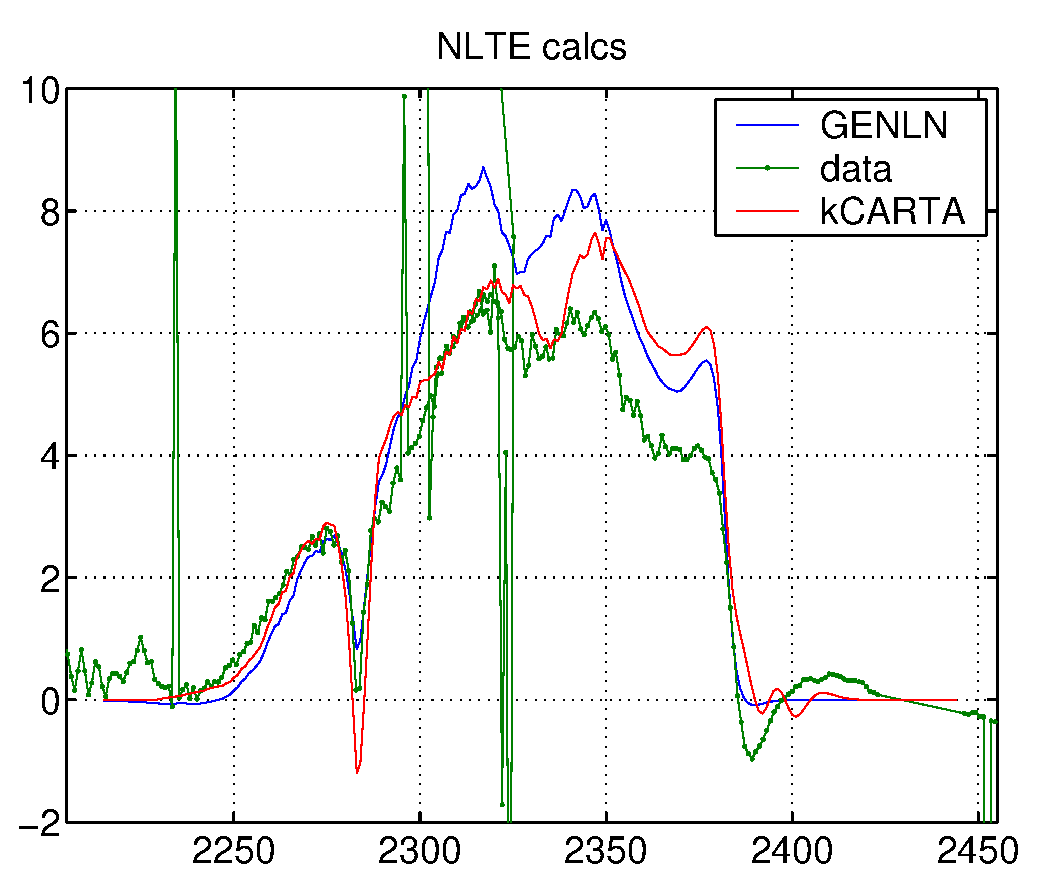
\includegraphics{/home/sergio/KCARTA/DOC/FIG/nlte.eps}
  \caption{Example of a NLTE computation using kCARTA and GENLN2}
  \label{fig:nlte} 
\end{figure} 

\section{TWOSTREAM scattering}

Time independent radiative transfer can be described by Schwartzchild's 
equation \cite{lio:80,goo:89}. As a beam propagates through a medium, the 
change in diffuse beam intensity $I(\nu)$ in a plane parallel medium is 
given by 
\[
\mu \frac{dI(\nu)}{dk_{a}} = -I(\nu) + J(\nu)
\]
where $\mu$ is the viewing angle, $k_{a}$ is the optical depth due to 
absorption, $\nu$ is the wavenumber and $J(\nu)$ is the source function. If 
the medium is nonscattering, such as would be expected in a ``clear sky,'' 
the source function is simply the Planck emission $B(\nu,T)$ at the
layer temperature $T$, implying that there is absoprtion attenuating the beam,
and  Planck emission from the layer adding to the beam. If we assume that the
temperature of the layer is constant, and that the incident intensity is 
$I(\nu,0)$, the equation is trivial to solve : 
\[
I(\nu,k_{a}) = I(\nu,0) e^{-k_{a}/\mu} + B(\nu,T)(1 - e^{-k_{a}/\mu})
\]
$1-e^{-k_{a}/\mu}$ is the emissivity $E$ of the layer, $e^{-k_{a}/\mu}$ is 
the transmission of the layer, and the reflection $R$ is 0. One can see that 
$R+T+E = 1$ in this simple case. Since the atmosphere is not isothermal, it 
is best modeled by dividing it up into layers thin enough that the 
temperature variation across each layer does not give significant 
spectroscopic variation between the layer top and bottom. Having obtained 
the one layer solution, it is trivial to propagate the radiation through 
successive layers and compute the radiation incident at the instrument. 

If the atmosphere is to be modeled more realistically, the effects of 
clouds and/or aerosols should be included. As above, there will be 
a reduction of the diffuse intensity $I(\nu,k_{e})$ by single scattering and
absorption (where $k_{e}$ is the extinction crosssection, which is the sum 
of absorption $k_{a}$ and scattering $k_{s}$ cross sections) 
\cite{lio:80,goo:89}
\[
\mu \frac{dI(\nu)}{dk_{e}} = -I(\nu)
\]
The layer Planck emission $B(\nu,T)$ still contributes to the source function 
$J(\nu)$. However, to maintain thermal equilibrium, only the absorptive 
portion of the extinction is included, and so the contribution to the
source term is now
\[
B(\nu,T) \frac{k_{a}}{k_{e}} = B(\nu,T) \left(1 - \frac{k_{s}}{k_{e}} \right) 
\]

In addition, we need to include scattering of diffuse intensities at 
other angles $\mu\prime$ into the viewing angle, which in three dimensions 
would be given by \cite{lio:80,goo:89}
\[
dI(\nu,\Omega,k) = k_{s} \mu \int_{4\pi} I(\Omega,\Omega\prime,k) 
P(\Omega,\Omega\prime) d(\Omega\prime)
\]
as well as the scattering of the direct solar beam into the viewing beam
\cite{lio:80,goo:89}
\[
dI(\nu,\Omega,k) = k_{s} \mu I_{sun}(\Omega,\Omega_{sun},k) 
P(\Omega,-\Omega_{sun}) 
\]
Here $P(\Omega,\Omega\prime)$ is the phase function, which gives the 
probability of scattering from solid angle $\Omega\prime)$ to solid angle
$\Omega$. The phase function and the extinction properties of the layer are
computed using electromagnetic theory; if one assumes that the particles are
spheres such as would be the case of raindrops in a cloud, then Mie theory 
\cite{van:82,lio:80,boh:98} can be used to determine these properties; if
one wants to describe the scattering properties of ice particles in a high
altitude cirrus cloud, one could use more elaborate ray tracing programs to 
determine these properties. 

If we consider  the azimuthally symmetric case, the phase function is now 
\cite{lio:80}
\[
P(\mu,\mu\prime) =  \frac{1}{2\pi} \int_{0}^{2\pi} 
P(\mu,\phi;\mu\prime \phi\prime) d\phi\prime
\]

Defining the single scattering albedo as
 $\omega_{0} = \frac{k_{s}}{k_{s}+k_{a}}$, and pulling together all of
the above, we finally have the radiative transfer equation to be solved 
\cite{lio:80,goo:89}
\[
\begin{array}{ccc}
\mu \frac{dI(\nu)}{dk_{e}} & = & I(\nu) - B(\nu,T)(1-\omega_{0}) - \\
& & 
\frac{\omega_{0}}{2}\int_{-1}^{+1} I(\nu,k_{e},\mu\prime) P(\mu,\mu\prime)
d(\mu\prime) - 
\frac{\omega_{0}}{4\pi} \pi I_{sun} P(\mu,-\mu_{sun}) e^{-k_{e}/\mu_{sun}} 
\end{array}
\]

This is an integrodifferential equation, which means that obtaining
the intensity at an arbitary viewing angle $\mu$ requires knowledge of the 
intensity at various angles, as one needs to perform an integral of these
intensities, weighted by the phase function. One way of evaluating the 
integral is by
Gaussian Legendre quadrature, which minimises the error in the integral by
picking a set of points over the $[-1,+1]$ interval. Depending on the number
of quadrature points chosen, we have an $n$ stream solution. Some scattering
packages such as \textsf{DISORT} and \textsf{CHARTS} allow the user to pick
the number of streams used. Others such as \textsf{RTSPEC} have a fixed 
number of streams. This should not be a very serious problem, as the large 
number of scatterers actually smooths out the phase function \cite{dee:98}, 
and a twostream solution can be quite accurate. The \textsf{RTSPEC} package
includes both the radiative transfer algorithm as well as Mie scattering code
to compute the particle scattering properties (more accurately, the scattering
properties of a distribution of particles). This package, as well as 
\textsf{DISORT} has been interfaced with \textsf{kCARTA}. 

To be able to compute the radiance when a cloud is present, as well as a 
solar beam, we also developed a simple multilayer \textsf{kTWOSTREAM} 
scattering package. This combines the twostream speed of \textsf{RTSPEC} and 
allows the user to include solar beam scattering (\textsf{DISORT} also allows
beam scattering, but is more slow). The atmosphere is divided up into three 
regions : clear from 
Top-Of-Atmosphere to CloudTop, cloudy, and clear from CloudBottom to Ground.
While simple clear sky radiative transfer is computed in the clear layers, the
reflection, transmission, emission and solar components at the twostream 
angles ($R,T,E,B$) and viewing angle ($r,t,e,b$) are computed for each cloudy
layer, with the layers being added together if the cloud is a multilayer one.
This gives the overall reflection, transmission, emission and beam 
scattering parameters of the cloud.
 
For both a downlook as well as an uplook instrument, we first compute the 
background thermal radiation that makes it down to the surface. 
When including the cloud layer in this initial computation, only the 
absorptive contribution of the cloud extinction depth is included. If the sun
is ``on'', a similar computation of the direct solar beam component at the
Earth's surface is performed. Together with surface emission, and the 
reflection of the background thermal and solar radiations, we propagate two 
beams back to the cloud bottom : one beam at viewing angle $\theta$ and a 
beam at the twostream angle $\arccos(1/\sqrt3)$. Similarly we compute the 
radiation incident downwards at the cloud top at stream angle 
$\arccos(1/\sqrt3)$ (and if necessary, the direct solar beam intensity that 
is incident at the cloud top, at solar angle $\theta_{sun}$). 

Having initialised the boundary conditions, we can propagate the up- and down-
going stream radiations (at $\pm arccos(1/\sqrt(3))$) throught the cloud, 
after which we can compute either the upgoing radiation at cloud top, or down 
going radiation at cloud bottom, at the viewing angle. The third and final 
stage is to compute the radiation to the instrument.

Since the sun creates a natural asymmetry in the radiative transfer, we 
choose to merge the cloud layers from top to bottom. Another point to mention 
is that we compute the reflection, transmission and emission coefficients for 
arbitrary viewing angle, and so a casual check of these coefficients would 
make it seem that $r+t+e$ is not energy conserving (i.e. is not 1). However, 
if one limits the computations to a viewing angle that corresponds to that of 
the two streams, then energy is indeed conserved ($R+T+E = 1$, the uupercase 
denoting the coefficients at the stream angles while the lower case denotes
them at arbitrary viewing angle). 

To agree with the clear sky outputs of \textsf{RTSPEC} and \textsf{DISORT}, 
the only layer temperature variation is exponential-in-optical depth in the 
cloudy layers; 
for the clear layers, we use the average temperature of the layer (which 
agrees very well with the linear-in-tau clear layer variation used in the 
above mentioned packages. However, depending on the wavenumber region, it is
apparent that the authors of the various scattering packages might need to 
agree on the exponential-in-tau variation both in cloudy and clear layers, as 
this could lead to brightness temperature differences of upto 0.6 K.

The layer addition is done in much the same fashion as is presented in Goody 
and Young \cite{goo:89}. The two stream equations are exactly solved for 
the layer in question (note that we define $k=0$ at the bottom of the 
layer, and that there is an implicit wavenumber dependence $\nu$) : 

\[
\begin{array}{ccc}
\mu_{+} \frac{dI^{+}}{dk} & = & -I^{+} + \frac{\omega_{0}}{2} 
(I^{+}(1 + 3g\mu_{+} \mu_{+}) + I^{-}(1 - 3g\mu_{+} \mu_{+})) + \\
                             & & B_{b}(1-\omega_{0})e^{\beta k} + 
\frac{\omega_{0}}{4}S_{T}e^{-(T-k)/\mu_{sun)}}P(\mu_{+},-\mu_{sun})
\end{array}
\]

\[
\begin{array}{ccc}
-\mu_{+} \frac{dI^{-}}{dk} & = & -I^{-} + \frac{\omega_{0}}{2} 
(I^{+}(1 - 3g\mu_{+} \mu_{+}) + I^{-}(1 + 3g\mu_{+} \mu_{+})) + \\
                            & & B_{b}(1-\omega_{0})e^{\beta k} + 
\frac{\omega_{0}}{4} S_{T} e^{-(T-k)/\mu_{sun}}P(-\mu_{+},-\mu_{sun})
\end{array}
\]

where we define
\[
\begin{array}{lcl}
\mu_{+}            & & \mbox{upgoing stream angle} \\
\mu_{-}            & & \mbox{downgoing stream angle} = -\mu_{+} \\
I^{+}              & & \mbox{upgoing stream intensity} \\
I^{-}              & & \mbox{downgoing stream intensity} \\
k               & & \mbox{optical depth} \\
$T$           & & \mbox{layer total optical depth (0 at bottom, T at top)} \\
\omega_{0}         & & \mbox{layer single scattering albedo} \\
$g$         & & \mbox{layer asymmetry factor} \\
B_{b}        & & \mbox{radiance at bottom of layer} \\
T_{b}        & & \mbox{temperature at bottom of layer} \\
T_{t}        & & \mbox{temperature at top of layer} \\
\beta        & & 1/T log_{e}(T_{t}/T_{b}) \\
S_{T}        & & \mbox{solar radiance at top of layer} 
\end{array}
\]

The homogeneous part of this set of coupled equations is easily solved, giving
the two eigenvalues for the two streams; the inhomogeneous part corresponding 
to the layer temperature variation and the solar beam incident on the top of 
the layer is also easily solved. The boundary conditions are the incident
upward radiance at the bottom of the layer, and the incident downward 
radiance at the top of the layer. With this information, the twostream 
problem is completely solved for one layer.

For a multilayer cloud, at each spectral point, one could make the intensities
continuous across layer boundaries. The drawback is that a potentially large 
matrix (depending on the number of layers the cloud occupies) would need to 
be inverted for each spectral point, making computations tedious. An 
alternative is to rewrite the exact solutions for one layer in terms of the 
monolayer reflection $R$, transmission $T$, layer 
emission $E$ and beam $B$ coefficients. One can show that $R+T+E = 1$ in this 
case. Having the solution for one layer, we can then add the layers together 
to obtain the solution for a multilayer cloud. It is easily appreciated 
that at each spectral point the only computations used in this multilayer 
model are simple multiplications and additions, instead of matrix inversions.

Using the two stream solution, the problem for arbitrary angles can now be 
solved. The radiative transfer equation in this case can be written as 
(for $\mu \geq 0$)

which can more easily be written as 
\[
\begin{array}{ccc}
\mu \frac{dI}{dk} & = & -I + J\prime(k,I^{+}(k),I^{-}(k))
\end{array}
\]

where $J\prime(k,I^{+}(k),I^{-}(k))$ is the (Eddington's second 
solution) source function

\[
\begin{array}{ccc}
J\prime(k,I^{+}(k),I^{-}(k)) & = & \frac{\omega_{0}}{2} \left(
(I^{+} + I^{-}) + 3g\mu \mu_{+}(I^{+} - I^{-}) \right) \\
                             & & B_{b}(1-\omega_{0})e^{\beta k} + 
\frac{\omega_{0}}{4}S_{T}e^{-(T-k)/\mu_{sun)}}P(\mu,-\mu_{sun}) \\
\end{array}
\]

Since we already know the solutions to the twostream radiances $I^{+},I^{-}$,
this general equation can be exactly solved as well. The solution can be 
written as
\[
\begin{array}{ccc}
I(k,\mu) = \left( I(0,\mu) + S_{up}(k) \right) e^{-k/\mu}
\end{array}
\]
where $S_{up}(k)$ is a term that includes the scattering from the twostream
radiances into the view angle stream, as well as layer emission and 
scattering from the solar beam into the viewing angle. A similar set of 
equations can be written and solved for $\mu \leq 0$. Having obtained the one
layer solution for arbitrary angles, we can rewrite the solutions in terms 
of the more general refection, transmission, emission and beam coefficients
$(r,t,e,b)$ and then add layers together for a complete solution. Note that 
because there is scattering from other beams into the viewing beam, $r+t+e$ 
is not necessarily equal to one in this general case. 

Since the code computes the twostream radiation incident at the top and
bottom of the multicloud layer, as well as the radiation incident at the
viewing angle, it can now propagate the twostream radiances through the cloud 
in either direction, and use that to compute the radiation exiting the cloud 
at the viewing angle. The final stage of the computation is to propagate the 
radiation through the remaining clear sky to the instrument.

\section{Case Study  : Comparing three scattering codes}

In evaluating the performance and accuracy of the three scattering codes 
included in our \textsf{kCARTA} package, we concentrated on the window regions
in the 10 $\mu m$ and 3.7 $\mu m$ regions. If there is no cloud present, an 
uplooking instrument would look clear into the cold sky in these regions.
However, even though the atmosphere is probably more transparant at 
3.7 $\mu m$ than at 10 $\mu m$, $Planck$ $\times$ $layer$ $emission$ combine 
to give a lower simulated brightness temperature at 10 $\mu m$, which means 
that $BT_{3.7} - BT_{10} \gg 0$. If a cloud is present, the spectral 
signature of the cloud would reduce this brightness temperature difference, 
potentially allowing one to identify cloudy situations. 

The cloud signature depends on factors such as type (ice versus water versus
aerosol type) and the average size and number of particles present; the 
variations in the spectral signature can assist in identifying what type 
of cloud is present. Using the Mie scattering code that is included in the 
\textsf{RTSPEC} package, one can understand the effects that for example 
spherical ice particles would have on the measured radiances. 
Figure \ref{fig:ext_alb_asy} plots the extinction 
optical depths, single scattering albedos and asymmetry factos for two 
ice particle distributions. The mean partice diameters of the two 
distributions are 1.0 to 50.0 $mu m$;  each has an $IcePath$ of 
$1.0 g m^{-2}$. Looking at the extinction depth in the 10.0 $\mu m$ window
region (from about 800 to 1000 \wn), one can readily see there is a sharp 
feature which would manifest itself on the measured radiance. Similarly, the 
single scattering albedo in this region is much less than one, and so a 
simple model, which just adds on the cloud extinction depth to the clear sky 
gas optical depth, can be expected to produxe simulation results that agree 
very well with data.  

These two points combine to lead one to the following conclusions. Without a 
cloud present, the transmittance of the atmosphere in this 10 micron window
region is close to unity. The presence of a cloud would reduce the 
transmittance more at the 800 \wn end than at the 1000 \wn end of the window.
Without a cloud present a downlooking instrument would see clear down to 
the surface, thus enabling a sounding of the temperature of the surface. With
the cloud present, the asymmetric reduction in transmittance would lead to a
lower brightness temperature measured at 800 \wn than at 1000 \wn, with the
cloud spectral signature between these two points. On the other hand, an
uplooking instrument would be able to penetrate to the upper levels of the
atmosphere if no cloud is present, which means the clear sky brightness 
temperatures would be quite low. The presence of a cloud would reduce this
transparecy and the measured radiance would only see closer to the ground 
(higher temperatures) at the 800 \wn end than at the 1000 \wn end. Evidently 
for both uplook or downlook instruments, the clarity of the obtained 
spectral signature would depend on the thickness of the cloud.

Conversely in the 3.7 $\mu m$ region, the asymmetry factor and especially 
the scttering albedo have both increased appreciably towards 1.0, and so a 
more complicated radiative transfer scattering model must be used. Due to
this, one cannot easily use similar reasoning to that above to make
some conjectures about the effects clouds would have on the measured 
radiances. In addition, solar beam scattering is far more important in this 
portion of the infrared.

\begin{figure}
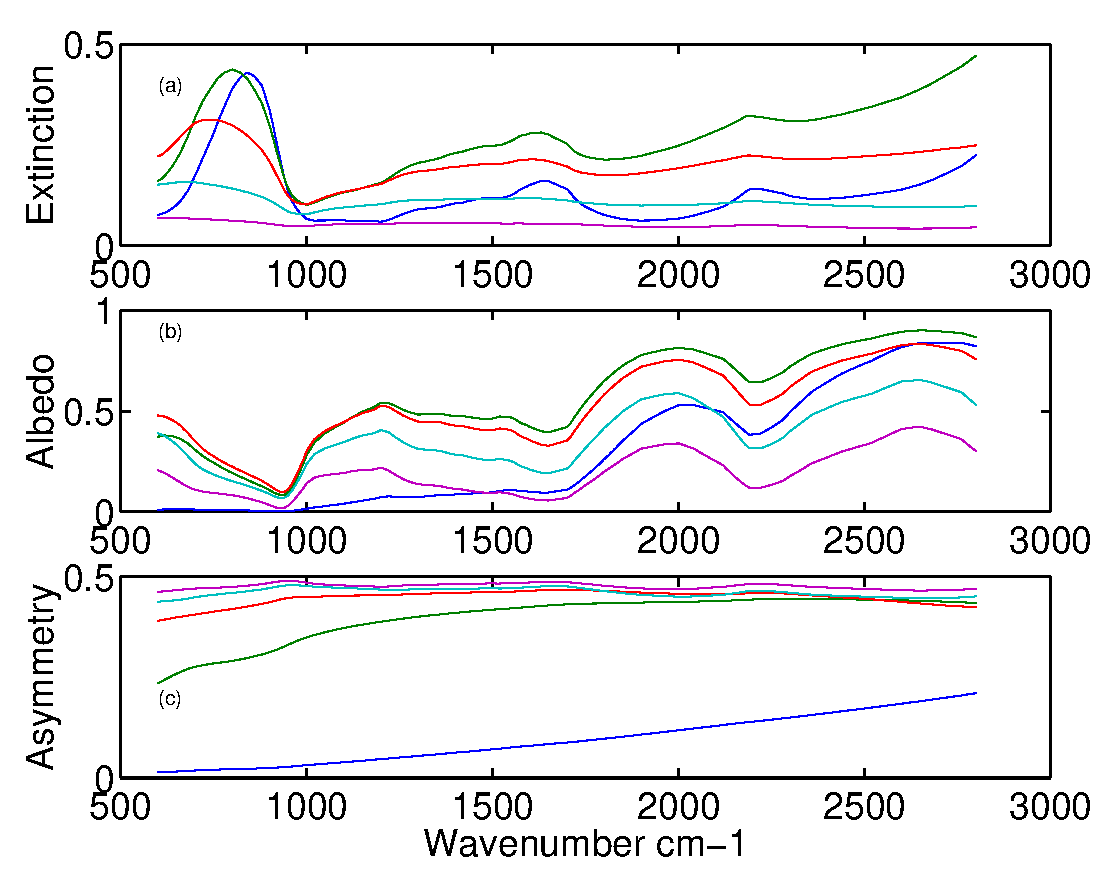
\includegraphics[width=6.0in]{FIG/ext_alb_asym.eps}
\caption{(a)Extinction optical depths (b) Single scattering albedos and 
(c) Asymmetry factors for five cirrus distributions of IcePath
1.0 $g m^{-2}$. Particles are spheres with mean diameters 1.0 (blue), 
5.0 (green), 10.0 (red), 20.0 (cyan), 40.0 (purple) $\mu m$.}
\label{fig:ext_alb_asy}
\end{figure}

Figure \ref{fig:uplook1} presents a series of \textsf{RTSPEC} simulations 
for an uplooking instrument on top of Mauna Laoa in Hawaii (695 mb), for a US 
Standard Atmosphere. The simulation is run for a nighttime clear sky, as well 
as for 1 km thick cirrus clouds of 1 $\mu m$ average particle size and 
varying IcePath, at a height of 10 km (220-240 mb). 
Figure \ref{fig:uplook40} does the same for cirrus clouds of 40 $\mu m$ 
average particle size and varying IcePath, at the same height of 10 km.

\begin{figure}
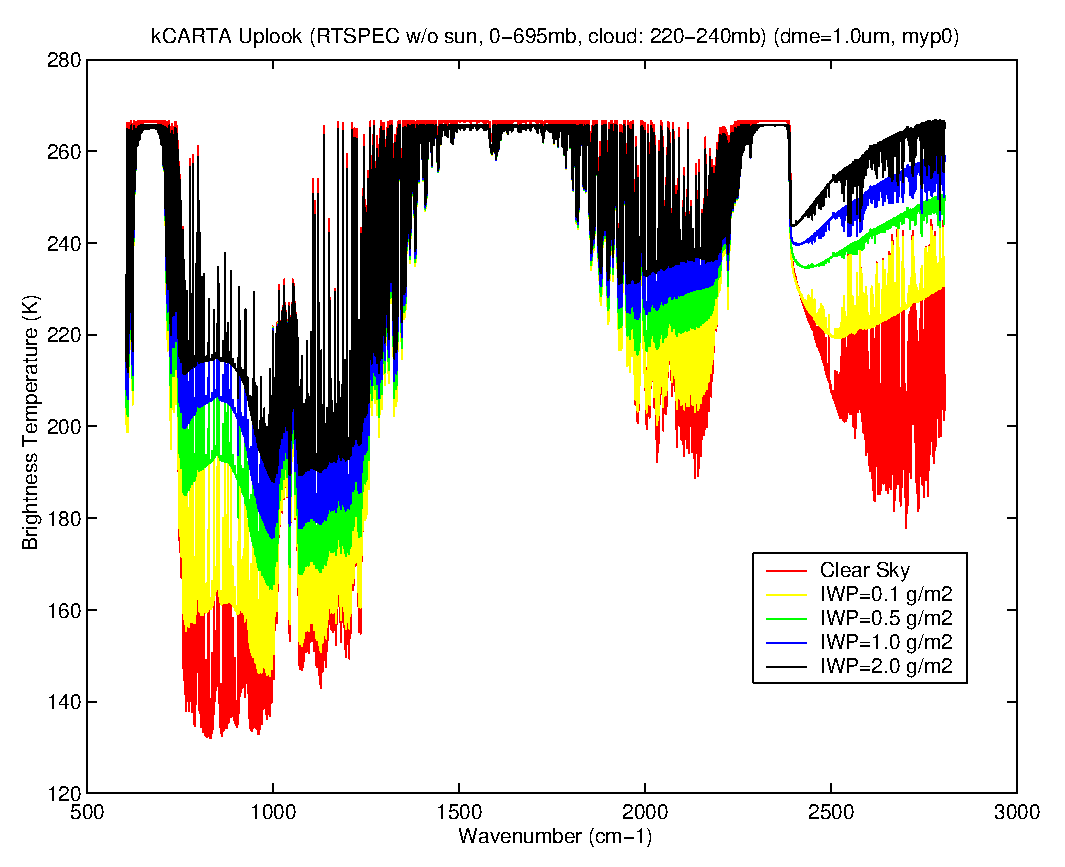
\includegraphics[width=5.5in]{FIG/1um.eps}
\caption{Uplook instrument \textsf{RTSPEC} simulations for cirrus clouds of
average particle diameter 1 $\mu m$}
\label{fig:uplook1}
\end{figure}

\begin{figure}
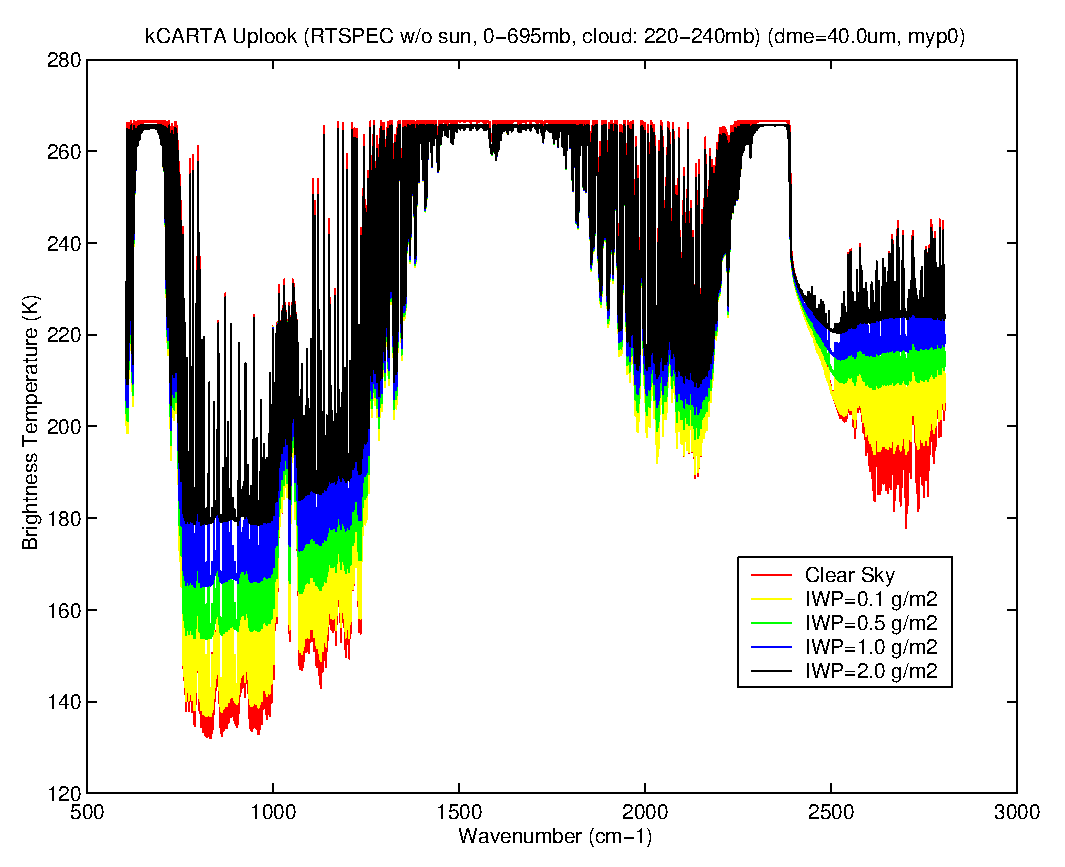
\includegraphics[width=5.5in]{FIG/40um.eps}
\caption{Uplook instrument \textsf{RTSPEC} simulations for cirrus clouds of
average particle diameter 40 $\mu m$}
\label{fig:uplook40}
\end{figure}

One can see that the 40 $\mu m$ particles have more scattering effects in the
2700 \wn range, compared to the 1 $\mu m$ particles; the brightness 
temperature is elevated much more in the former case, for the same IcePath. 
Conversely in the 1000 \wn region, the 1 $\mu m$ particles have much more of 
a spectral signature than the 40 $\mu m$ particles. Similar plots and 
reasoning would apply for a downlooking instrument.

To evaluate the three sets of scattering codes, we performed a series of tests
for 6 profiles (US Standard, Tropical, MidLatitude Summer, Midlatitude Winter,
SubArtic Summer, SubArtic Winter). 1 km thick cirrus clouds were typically put
in at a base height of 10 km, and the uplook and downlook radiances computed 
by \textsf{DISORT},\textsf{RTSPEC} and \textsf{kTWOSTREAM} for a variety of 
test scenarios such as instrument in space, or instrument on board an 
aircraft, were compared against each other. The atmospheres included being 
defined from (TOA = 0 mb, GND = 1013 mb) to (TOA = 50 mb, GND = 900 mb). The 
clouds had ice particles ranging from 1 to 40 $\mu m$ in size, with ice paths 
varying between 0.1 to 2.0 $g m^{-2}$, meaning they varied from sub visble to
almost opaque. 

In the window regions, looking in between the lines, with no 
sun on, the three methods typically differed by no more than 3K, both for 
downlook or uplook instruments. In the opaque regions, such as the ozone and 
water regions, there could be larger differences, especially for an uplook 
instrument. With the sun on, differences between by \textsf{DISORT} and 
\textsf{kTWOSTREAM} could begin to get as large as 5K, depending on the 
IcePath/Particle Size combination. Figure \ref{fig:solar_uplook_20um} plots 
the brightness temperature difference between \textsf{DISORT} and 
\textsf{TWOSTRM} for a typical uplooking instrument (mean particle diameter 
of 20 micron), while Figure \ref{fig:solar_downlook_1um} plots the 
brightness temperature difference between \textsf{DISORT} and 
\textsf{TWOSTRM} for an downlooking instrument (mean particle diameter 
of 1 micron). In both plots the differences start to get larger in the region
where the solar beam has an effect; with the solar beam off, the differences
between the two codes is that typical of the rest of the plot (less than 1.5 K
for a downlook instrument, less than 3 K for an uplook instrument).
Typical worst case results have been plotted (1 micron particles for a 
downlook instrument, and 20 micron particles for an uplook instrument). 

It should be remembered that even though \textsf{TWOSTR} is run at the 
monochromatic point spacing, while the radiative transfer computations for 
\textsf{DISORT} are done once every 20 points and then interpolated, the
twostream code is about four times faster. Similar comparisons between
\textsf{DISORT} and \textsf{RTSPEC} (with the sun off) were obtained.

\begin{figure}
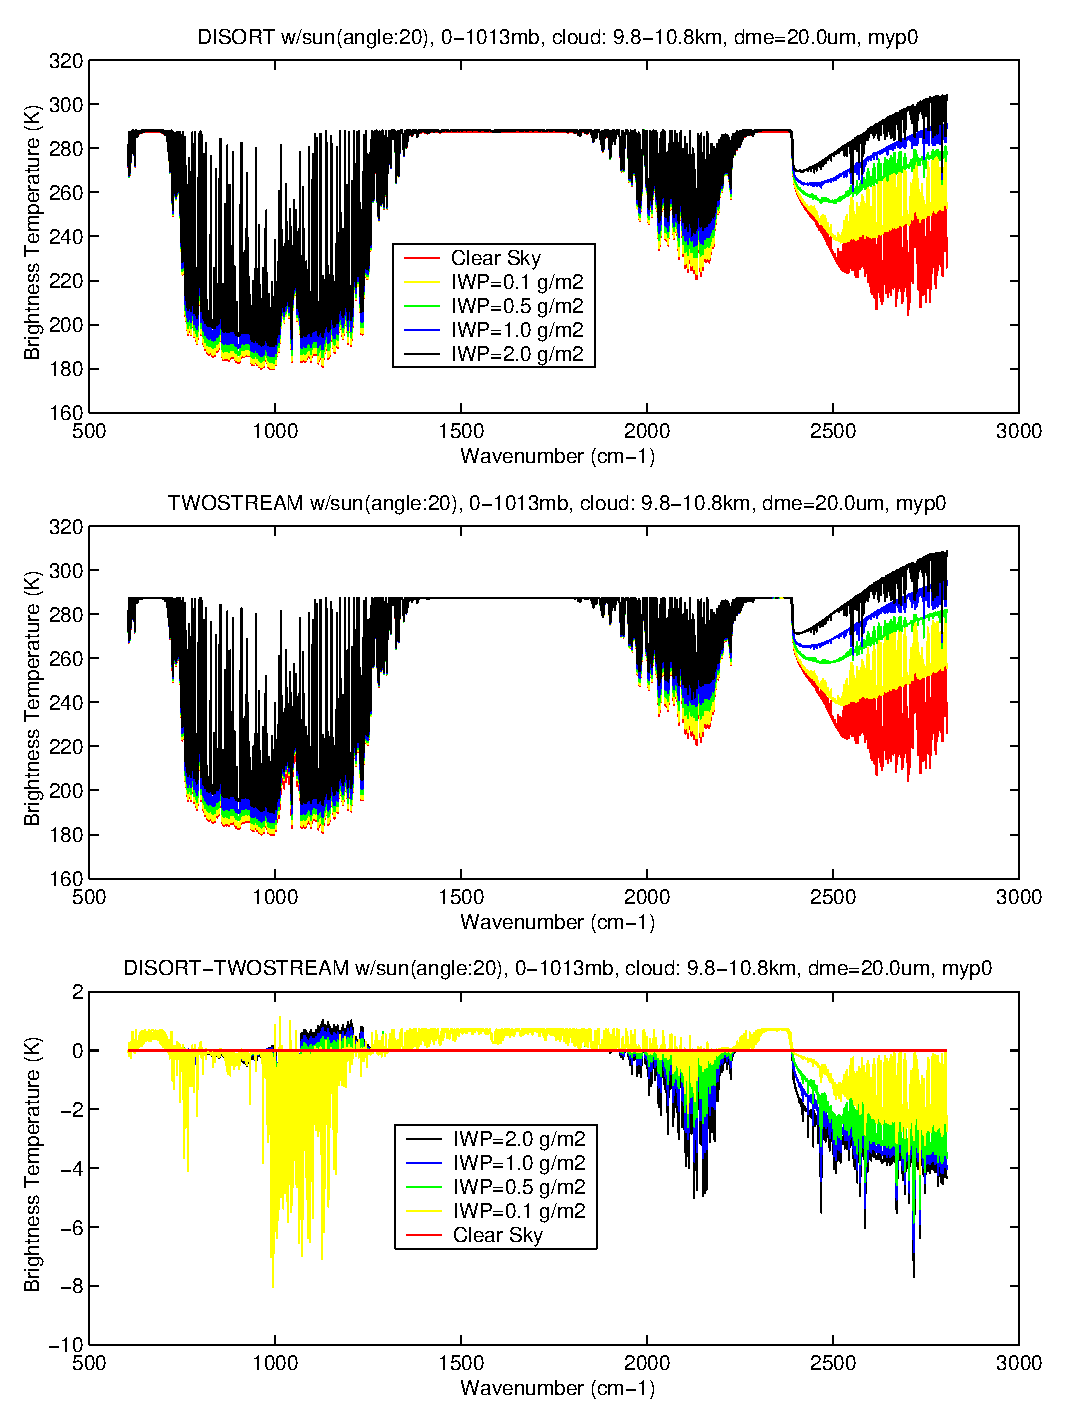
\includegraphics[width=5.0in]{FIG/14.eps}
\caption{Uplook instrument simulations for cirrus clouds of average particle 
diameter 20 $\mu m$} 
\label{fig:solar_uplook_20um}
\end{figure}

\begin{figure}
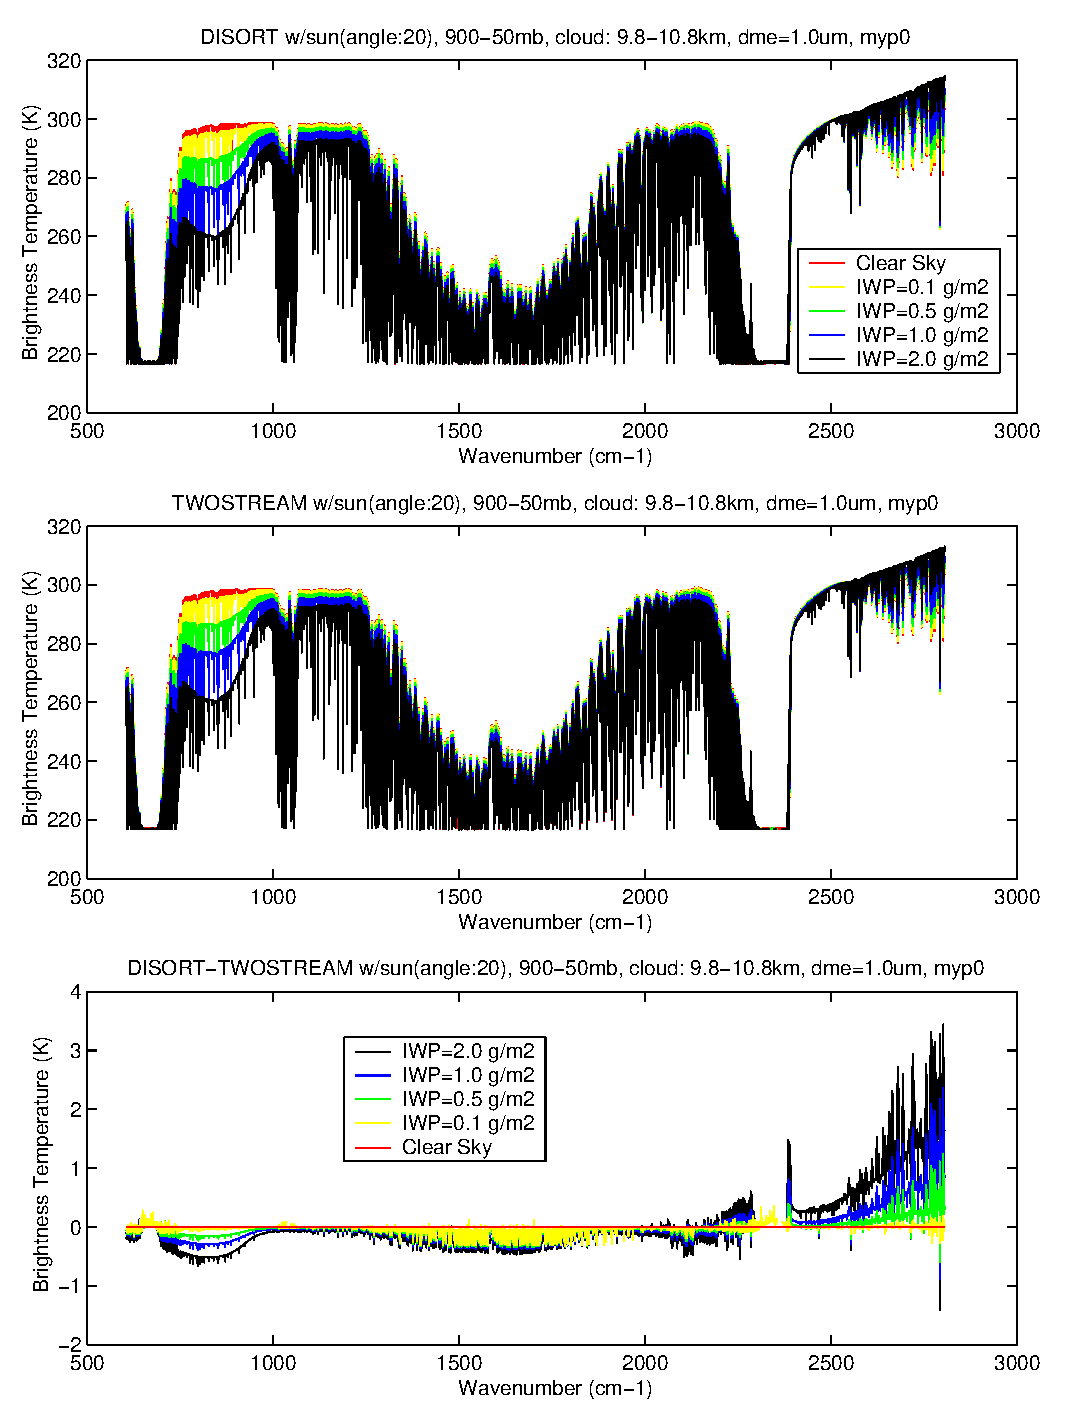
\includegraphics[width=5.0in]{FIG/61.eps}
\caption{Downlook instrument simulations for cirrus clouds of average 
particle diameter 1 $\mu m$}
\label{fig:solar_downlook_1um}
\end{figure}

\section{Conclusions}
Scattering effects due to clouds and/or aerosols can easily be 
included, using one of three scattering codes. While \textsf{DISORT} is a 
standard and well tested package that can include the effect of solar beam 
scattering, it is much slower than another package \textsf{RTSPEC}; however
this does not include the effects of beam scattering. Our =textsf{TWOSTR}
package is rapid and can include the effects of beam scattering, and has been
satisfactorily tested against \textsf{DISORT}.

\section{Acknowledgements}
This work was supported in part by NASA grant number 05-5-28045. We wish to 
thank users of kCARTA that have provided us with feedback. Ji Gou of UMBC 
performed multiple runs of \kc, to assess the different scattering codes. 
Dave Tobin of UW-Madison was instrumental in helping develop the \cd 
linemixing code, as well as modifying the water continuum coefficients. Dave 
Edwards of NCAR provided the {\sf GENLN2} line-by-line code to test the 
{\sf kCompressed} database against, allowed us to use modifications of some of 
his subroutines in {\sf KCARTA}, as well as helped us debug the NLTE code. 
In addition we thank Pat Arnott of the 
Desert Research Institute for motivating discussions about the applicability 
of a single scattering versus twostream approach, Frank Evans of the 
University of Colorado for help in getting RTSPEC interfaced, and Istvan 
Laszlo of University of Maryland, College Park for help in interfacing 
DISORT.

\bibliographystyle{unsrt}
\bibliography{/home/sergio/PAPERS/BIB/atmspec2002}

\end{document}

